\section{Ejercicio 4}
La asortatividad/homofilia es la tendencia de un nodo, de una red, se conecte con otros 
de caracteristicas similares, esto en terminos mathematicos es evaluar la correlaci\'on
de links entre nodos del mismo tipo \citep{newman2003}. Esta propiedad tiende a ser caracteristica 
para tipos de redes distintas: En redes de amistad por ejemplo se tiende a hacer uniones entre
nodos \textit{parecidos}, mientras que en redes biologicas, los \textit{hubs} tienes a evadirse 
entre ellos y asociarse con nodos de menor grado \citep{newman,barabasi}. 

En este ejercicio se plantea evaluar la asortatividad de cuatro redes (dos sociales y dos biol\'ogicas) a trav\'es
de dos m\'etodos distintos: Mediante la estimaci\'on de la correlaci\'on de grado a partir del grado medio del
vecindario de un nodo \citep{barabasi}; y a trav\'es del Coeficiente de Correlaci\'on de Grado propuesto por Newman
\citep{newman2003,newman}.

\subsection{Consideraciones generales}
\begin{figure}[!ht]
    \centering
    \begin{subfigure}[b]{0.30\columnwidth}
        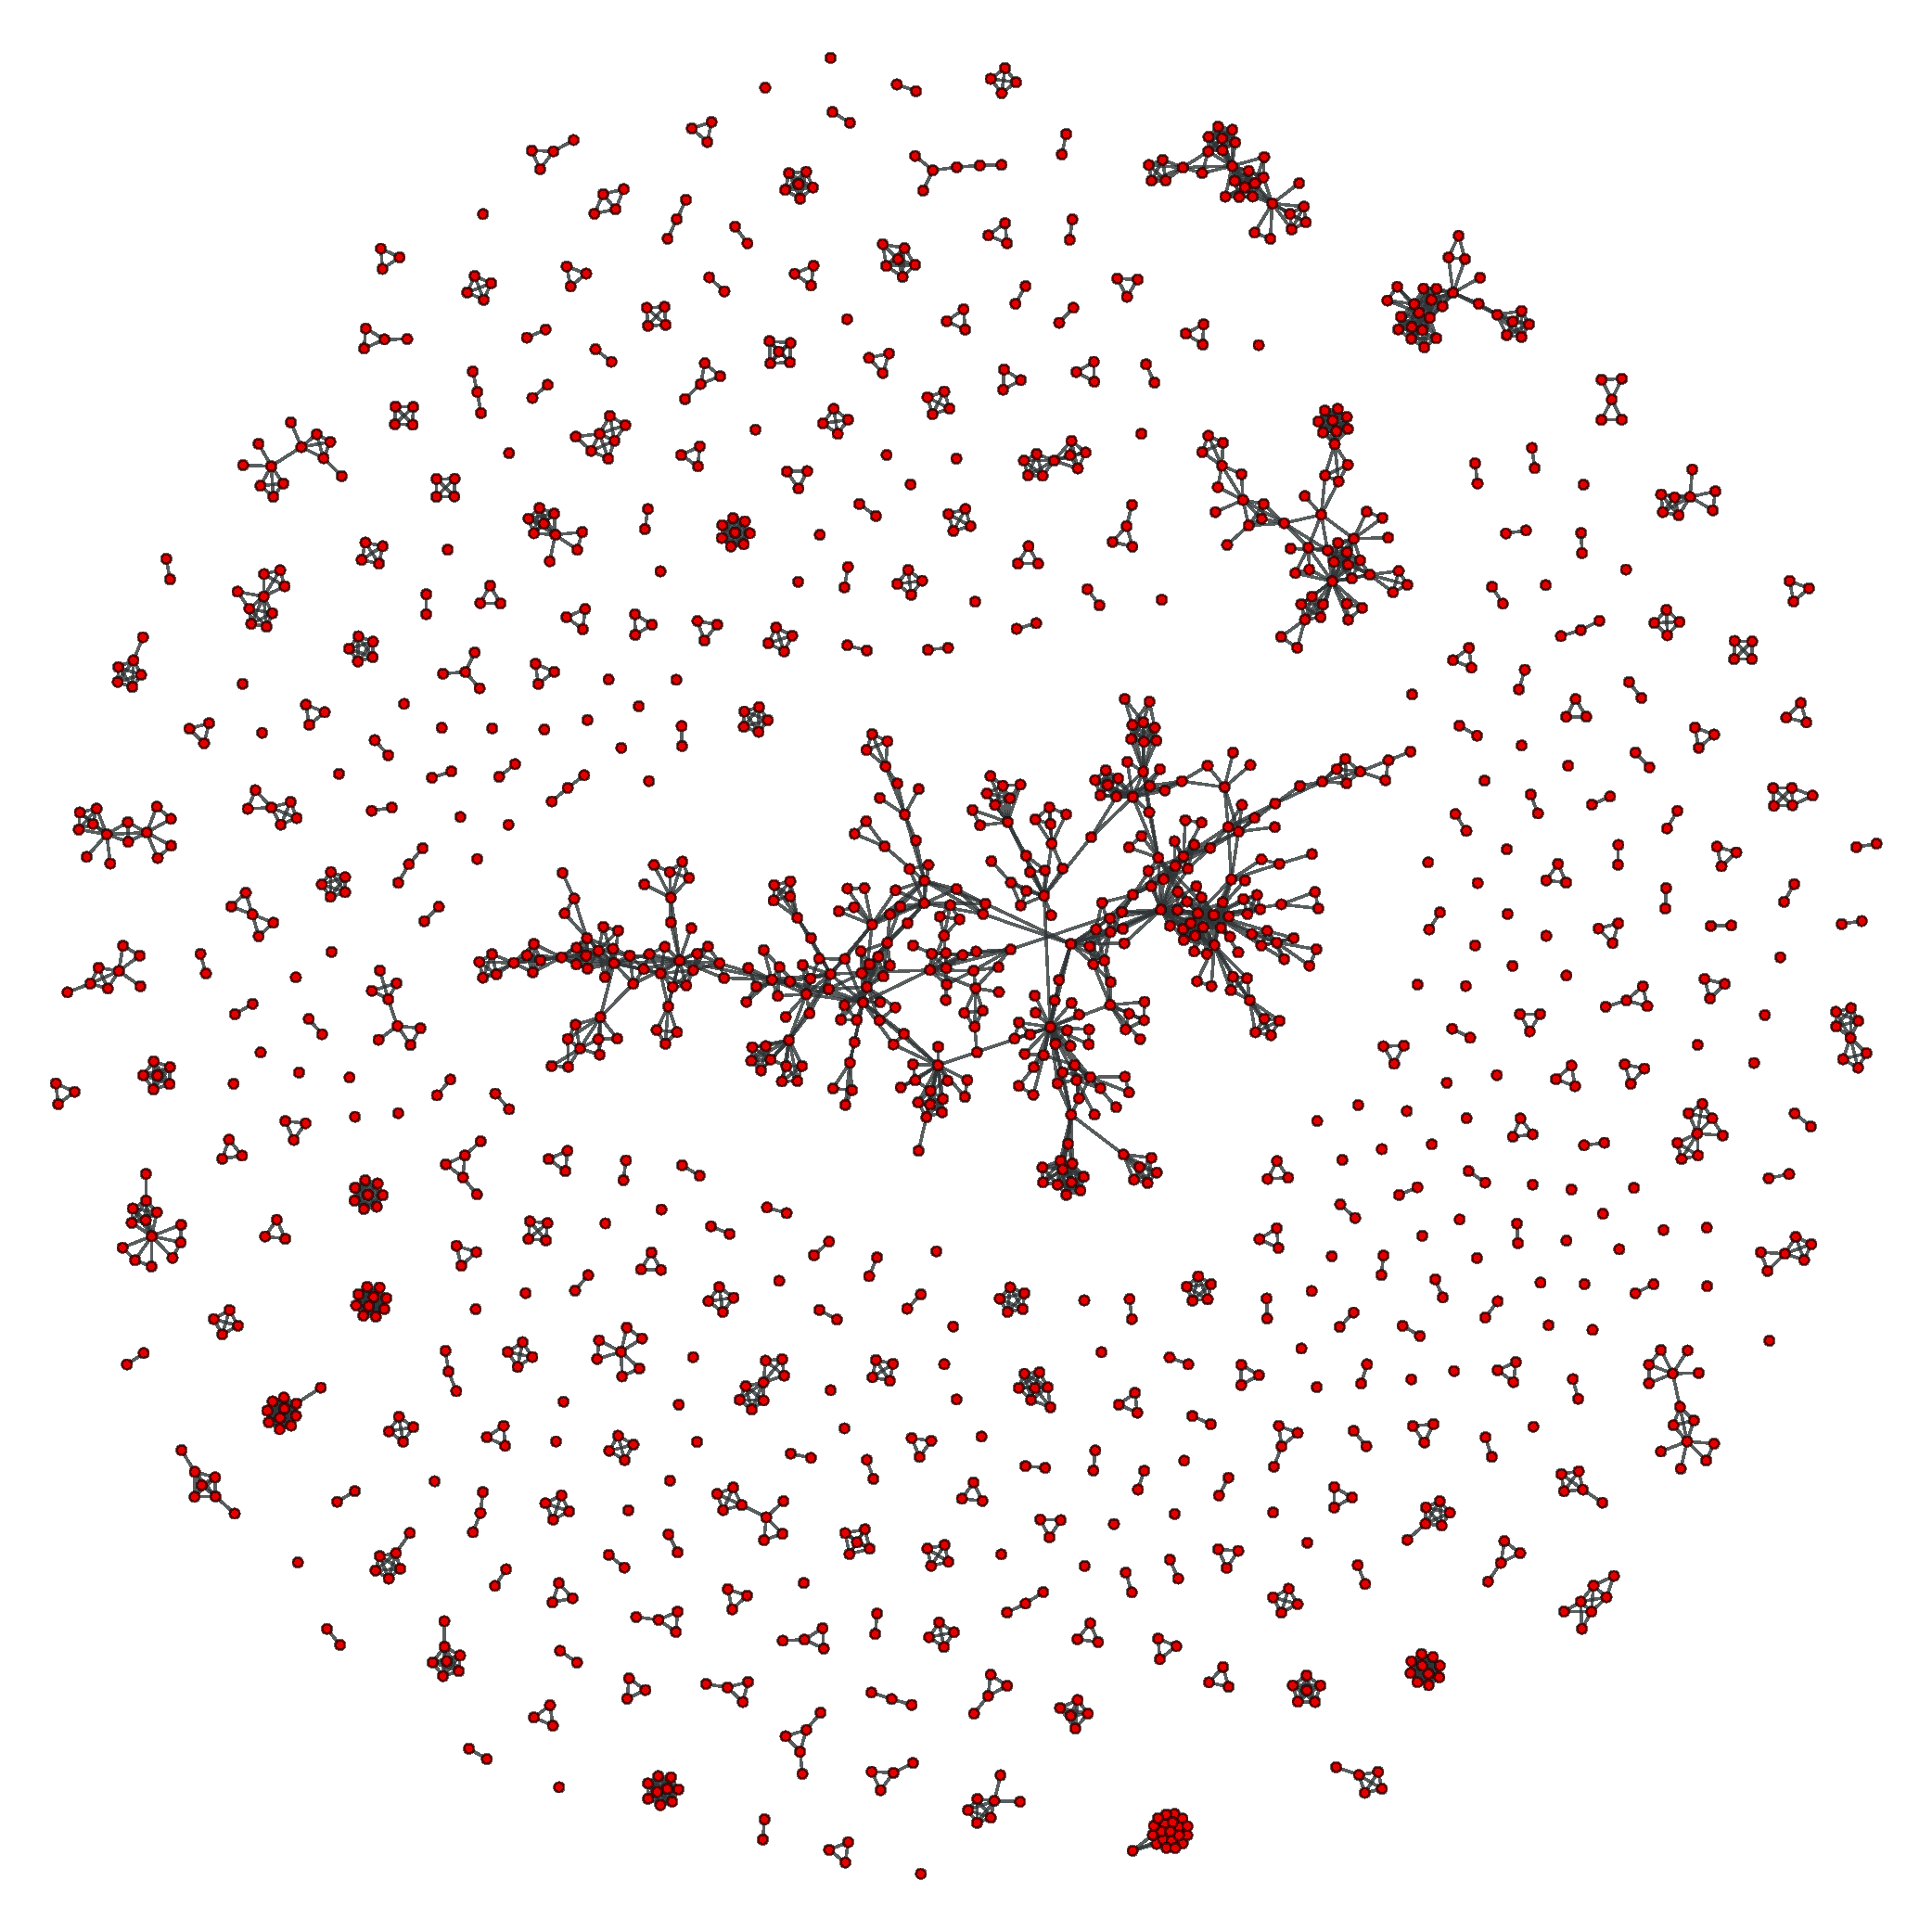
\includegraphics[width=\textwidth]{./schemes/netscience-gml.pdf}
        \caption{\label{fig4:NETSCIENCE}NETSCIENCE}
    \end{subfigure}
    \begin{subfigure}[b]{0.30\columnwidth}
        \includegraphics[width=\textwidth]{./schemes/as-22july06-gml.pdf}
        \caption{\label{fig4:INTERNET}INTERNET}
    \end{subfigure}
    \\
    \begin{subfigure}[b]{0.30\columnwidth}
        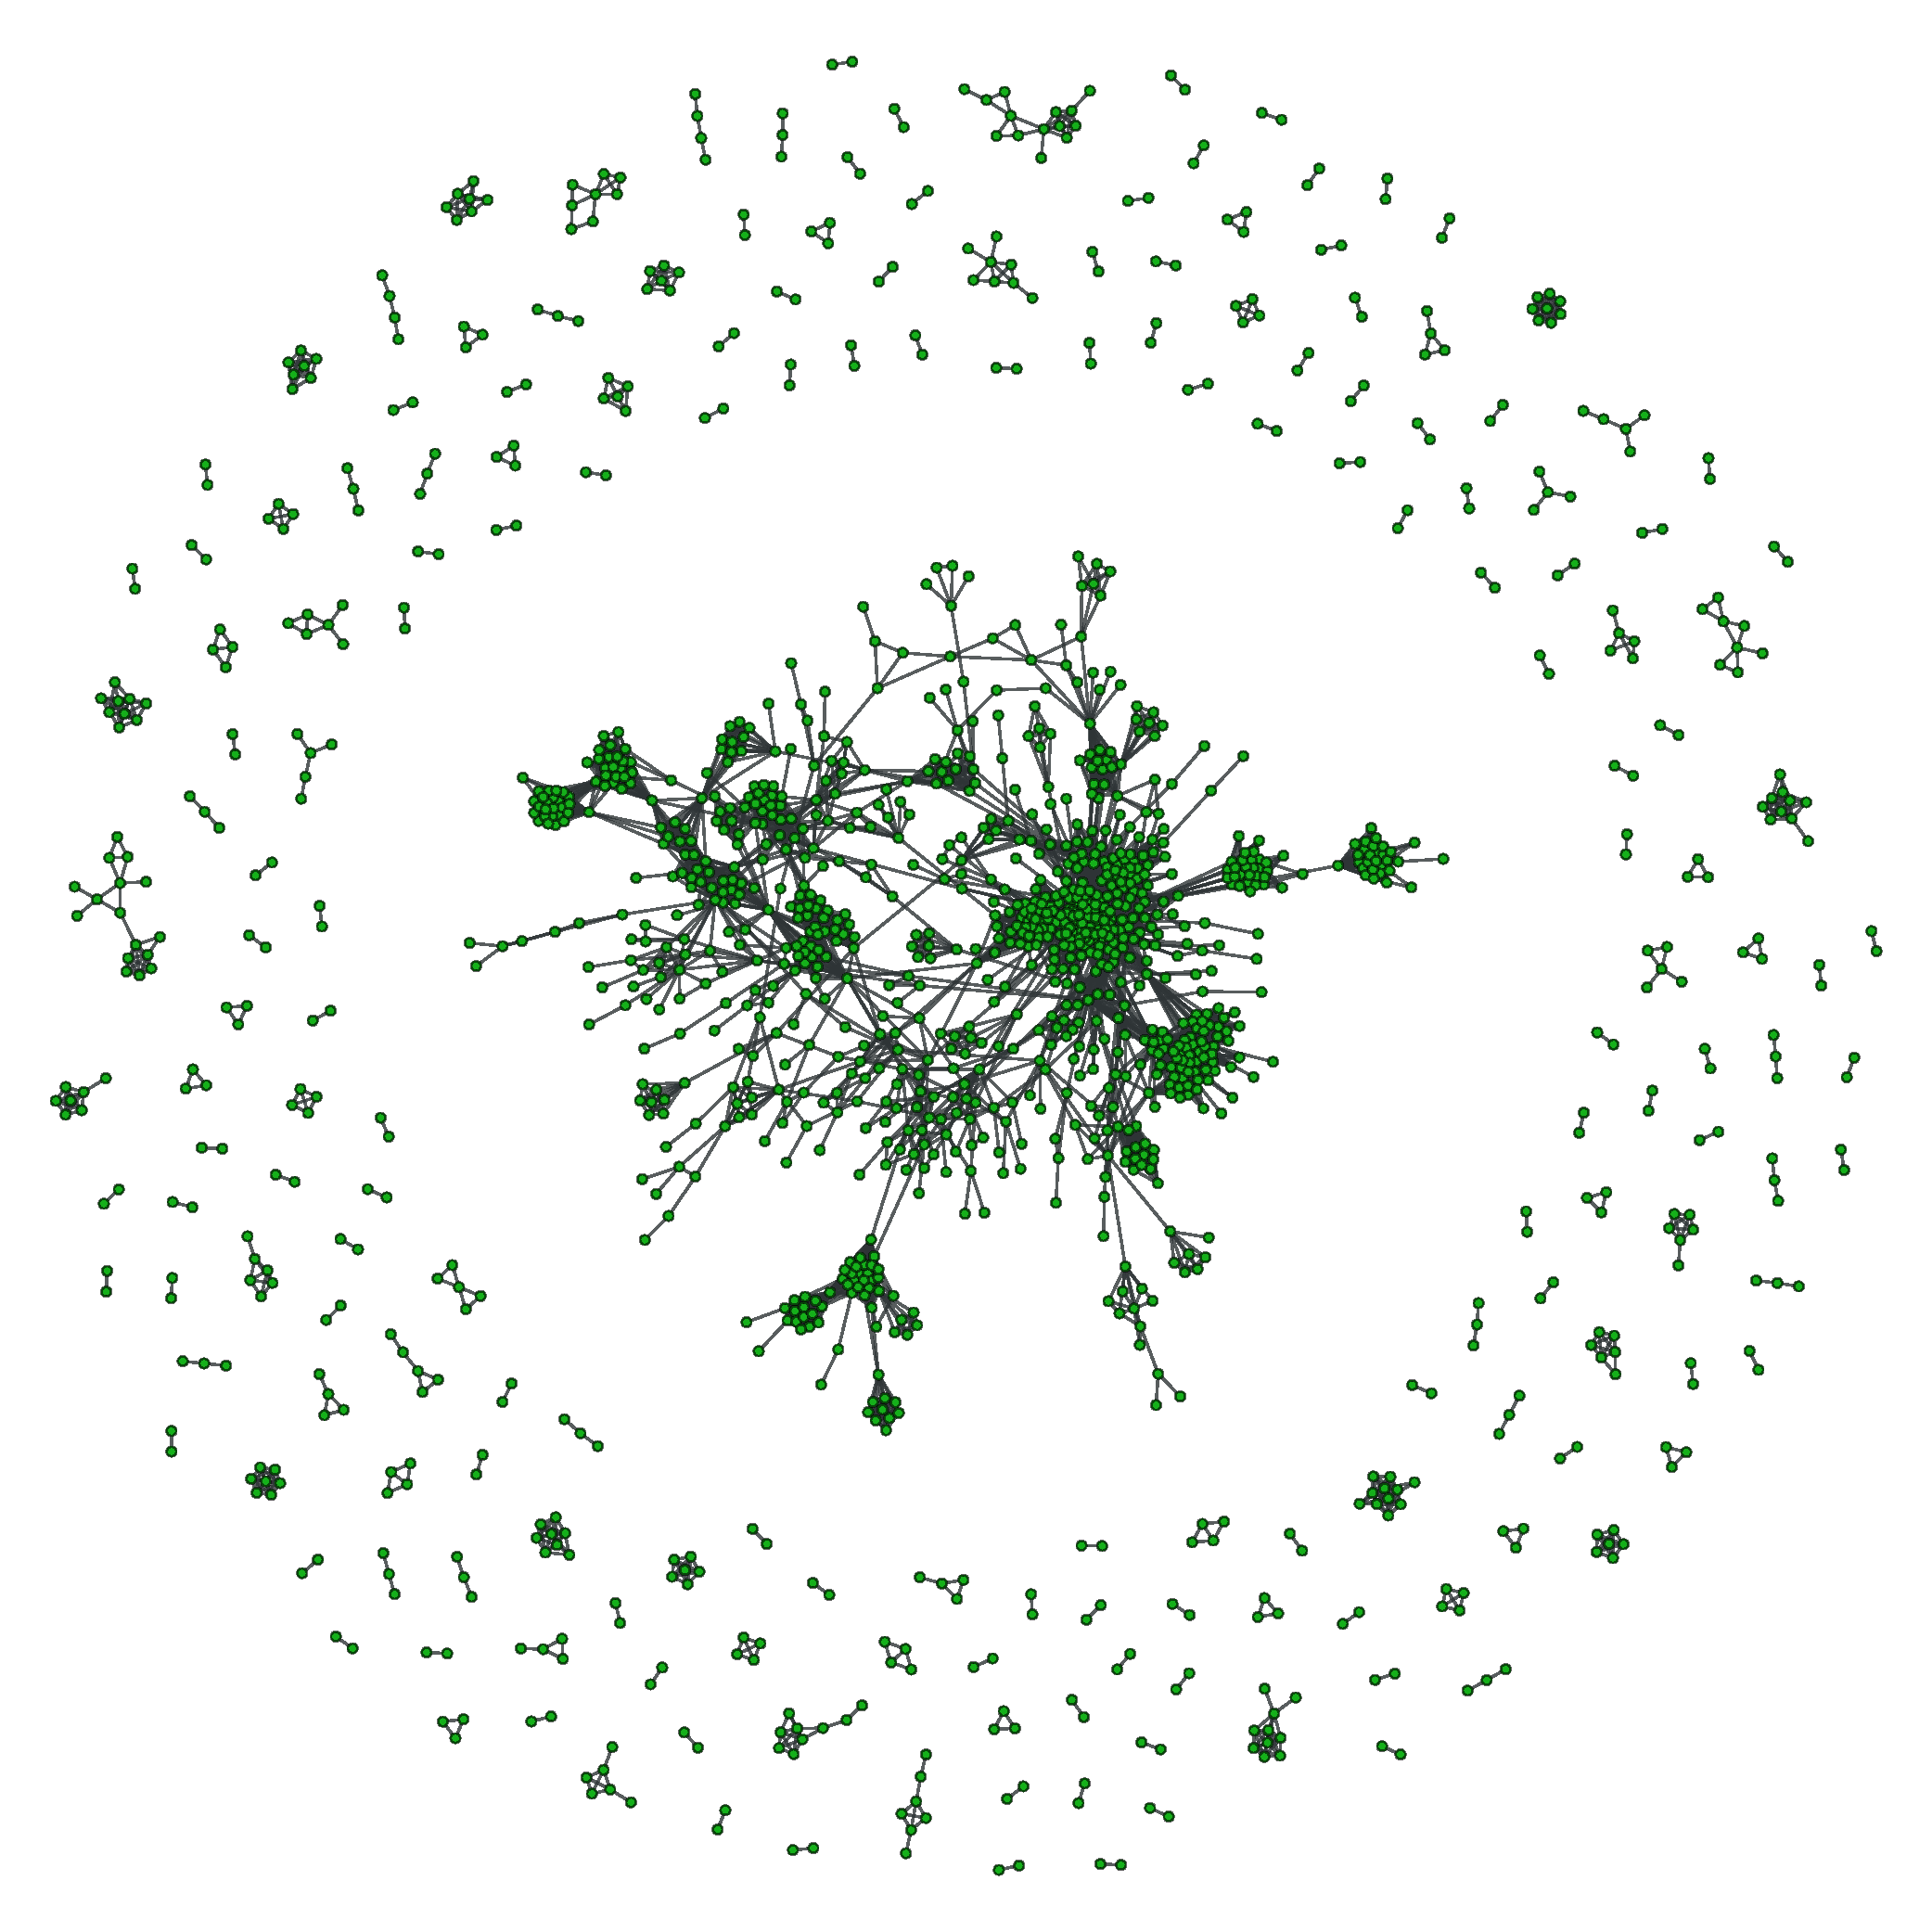
\includegraphics[width=\textwidth]{./schemes/yeast_AP-MS-txt.pdf}
        \caption{\label{fig4:ap_ms} AP-MS}
    \end{subfigure}
    \begin{subfigure}[b]{0.30\columnwidth}
        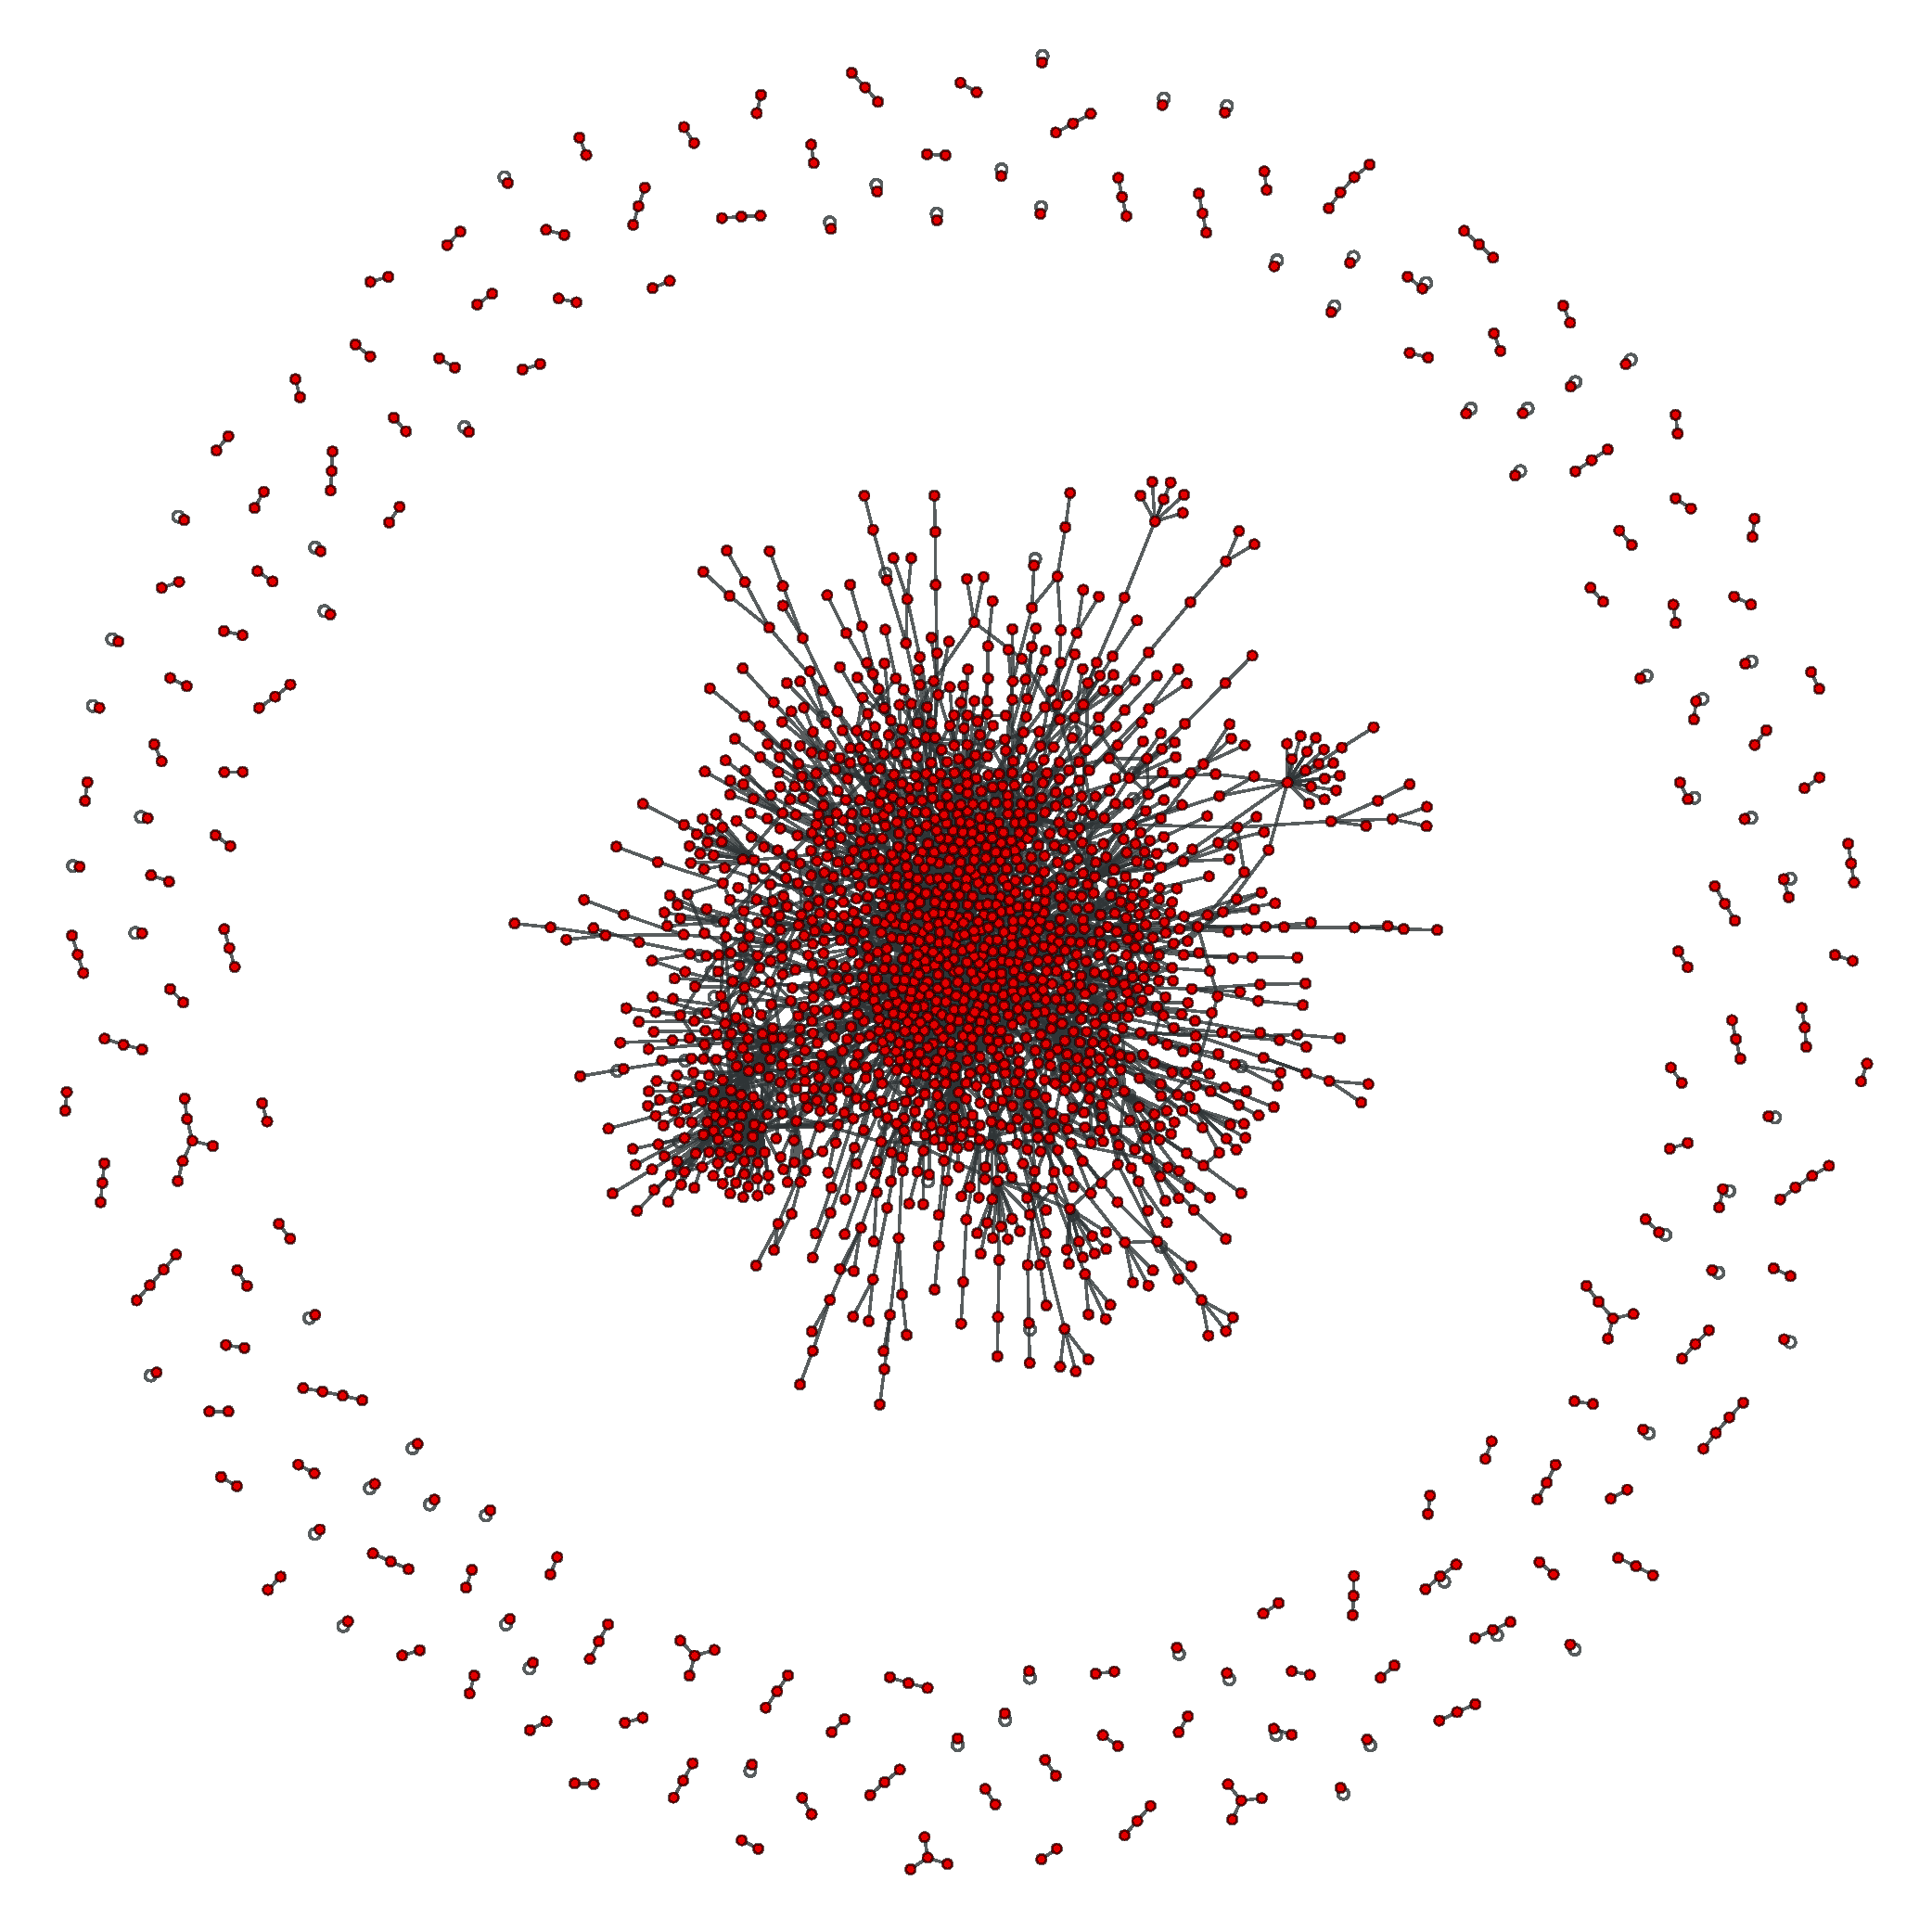
\includegraphics[width=\textwidth]{./schemes/yeast_Y2H-txt.pdf}
        \caption{\label{fig4:y2h} Y2H}
    \end{subfigure}
    \caption{\label{fig4:grafos}\textit{Layout} SFDP para cada red estudiada \\
    (script \texttt{plot.py~<archivo>\quad-f <fmt>}).}
\end{figure}
Consideremos las redes de colaboraciones cientificas (NETSCIENCE), red de internet (INTERNET) y dos redes de levadura analizadas 
en el ejercicio 1 (AP-MS y Y2H), las cuales son mostradas en la figura \ref{fig4:grafos}.


Un m\'etodo alternativo para 
evaluar asortividad es analizar la matriz de correlaci\'on entre grados (\textit{mixing matrix}) la cual se presenta en
la figura \ref{fig4:mix}.


\begin{figure}[!ht]
    \centering
    \begin{subfigure}[b]{0.45\columnwidth}
        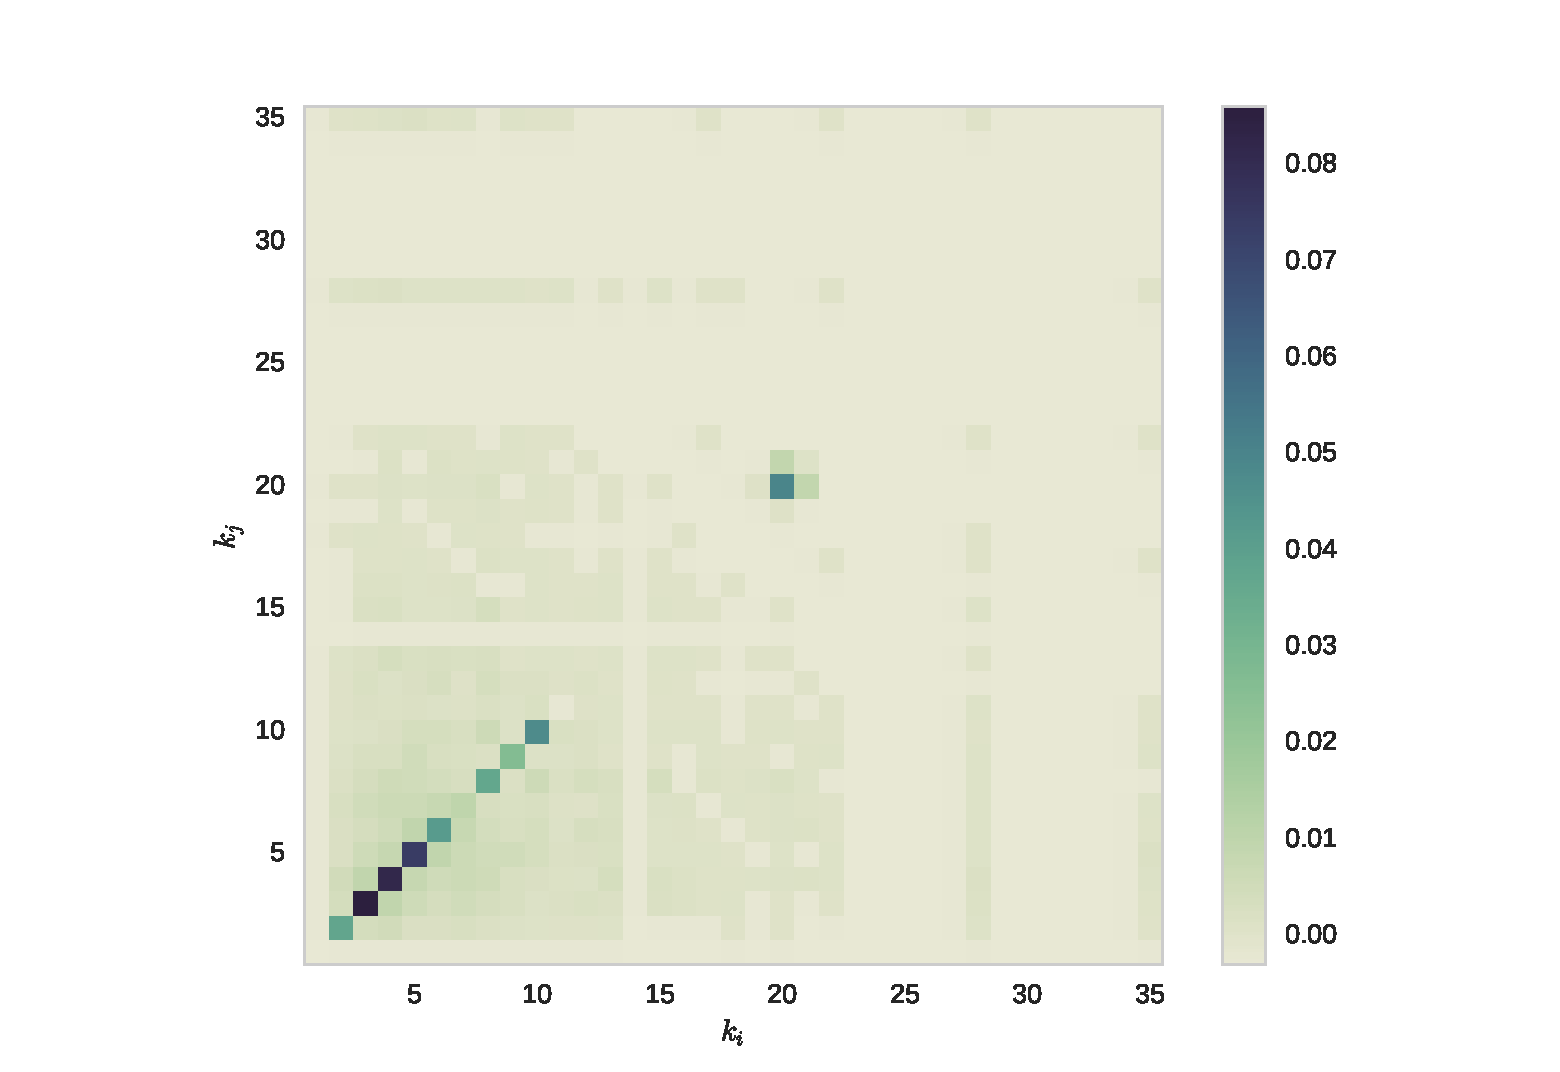
\includegraphics[width=\textwidth]{./schemes/mixing_netscience-gml.pdf}
        \caption{\label{fig4:NETSCIENCE}NETSCIENCE}
    \end{subfigure}
    \begin{subfigure}[b]{0.45\columnwidth}
        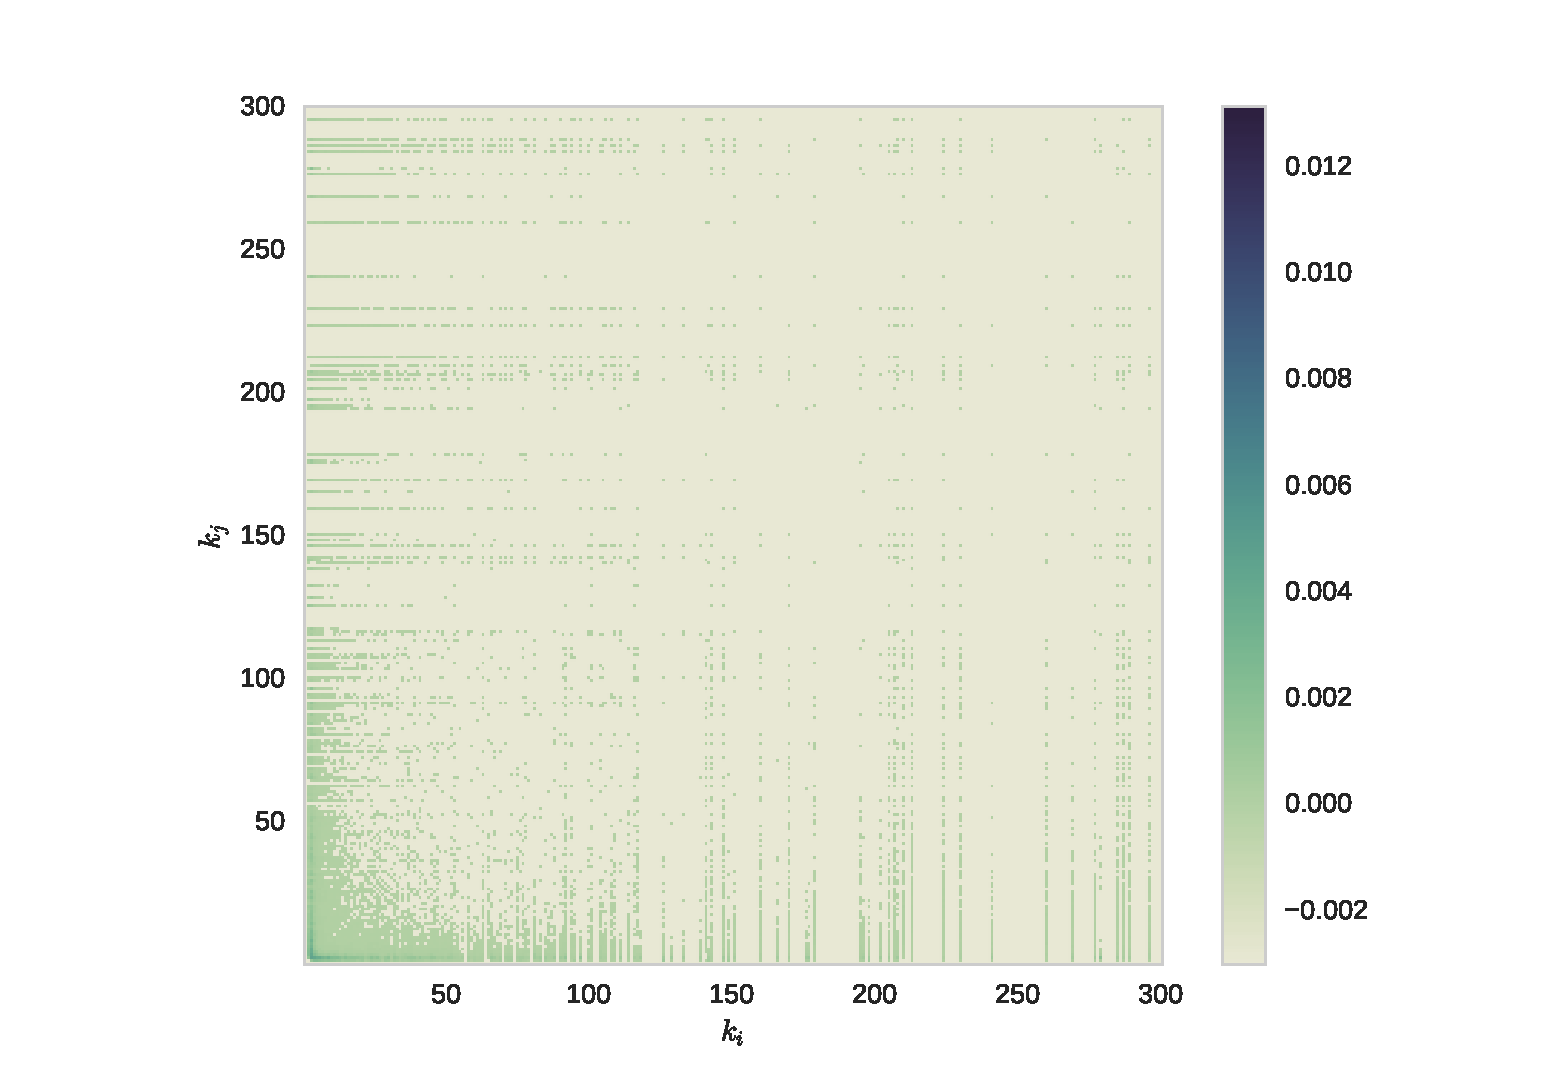
\includegraphics[width=\textwidth]{./schemes/mixing_as-22july06-gml.pdf}
        \caption{\label{fig4:INTERNET}INTERNET}
    \end{subfigure}
    \\
    \begin{subfigure}[b]{0.45\columnwidth}
        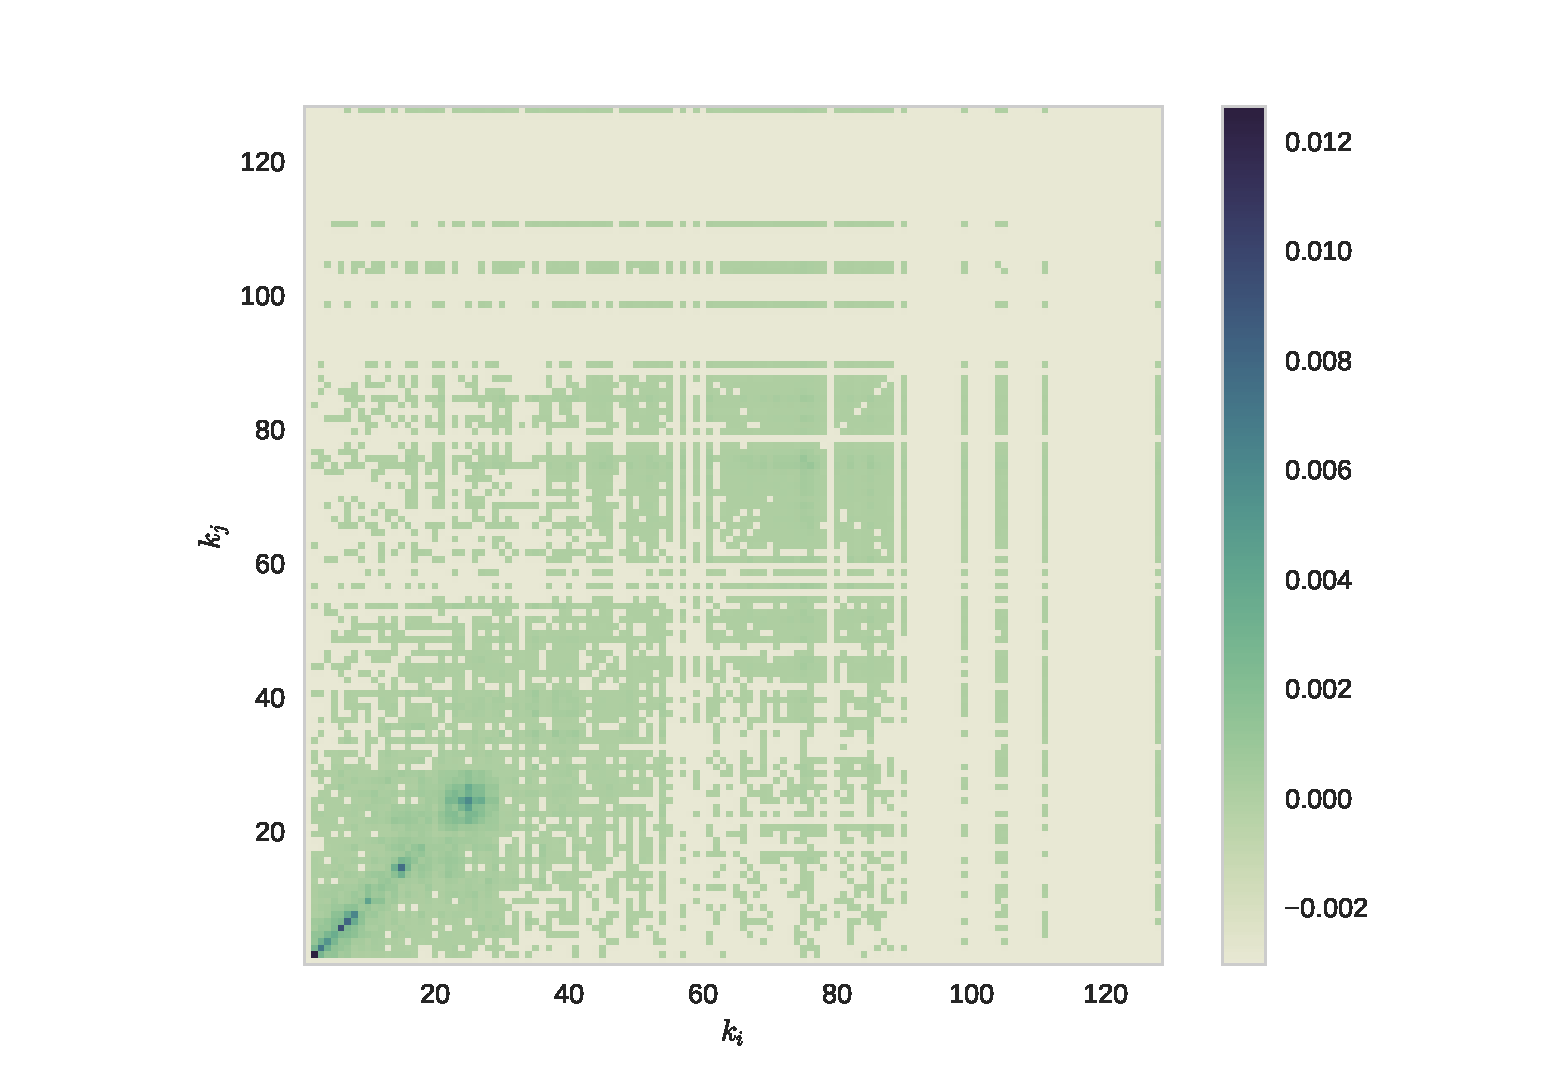
\includegraphics[width=\textwidth]{./schemes/mixing_yeast_AP-MS-txt.pdf}
        \caption{\label{fig4:ap_ms} AP-MS}
    \end{subfigure}
    \begin{subfigure}[b]{0.45\columnwidth}
        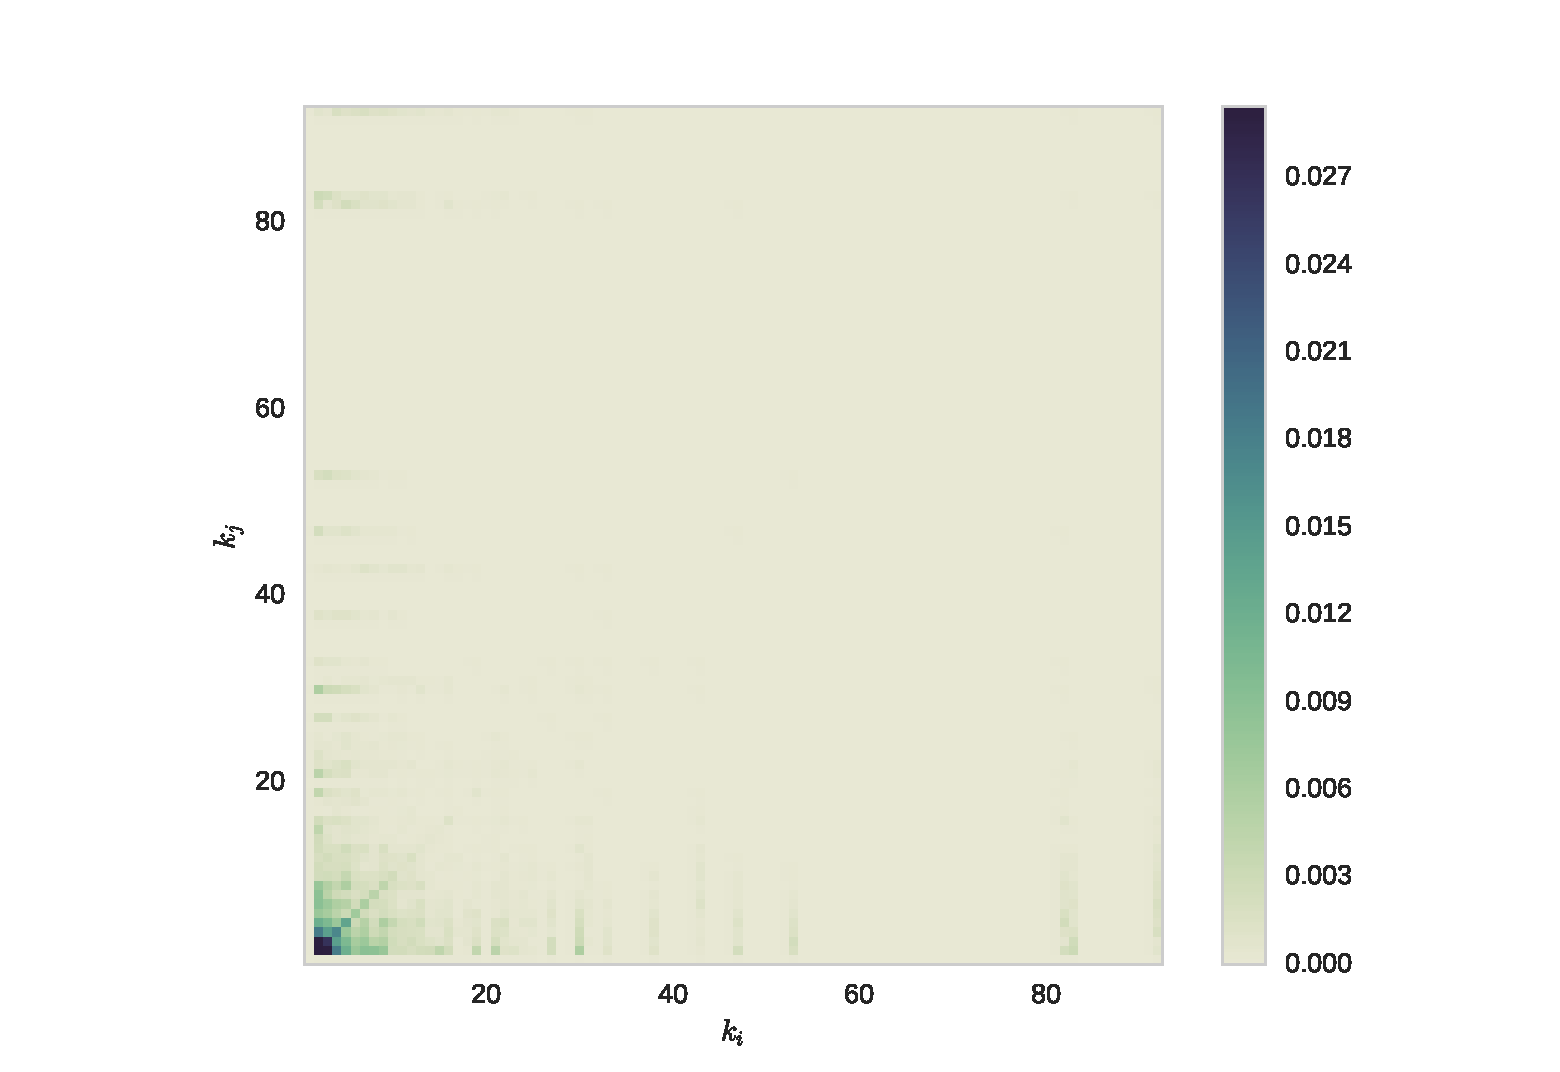
\includegraphics[width=\textwidth]{./schemes/mixing_yeast_Y2H-txt.pdf}
        \caption{\label{fig4:y2h} Y2H}
    \end{subfigure}
    \caption{\label{fig4:mix} Mixing Matrix para cada caso. En la red INTERNET se ha ajustado los limites de gr\'afico
    de manera que sean visibles las correlaciones de bajo grado
    \\(script \texttt{degree\_mixing\_plot.py <archivo>\quad-f <fmt>})}
\end{figure}

De la figura se puede observar que, para todos los casos, la mayor densidad de correlaci\'on se puede encontrar en los 
grados peque\~nos, y para NETSCIENCE y AP-MS parece seguir un comportamiento lineal (\textit{hubs} conectados 
con \textit{hubs}), mientras que en las redes INTERNET y Y2H se puede observar que los nodos de alto grado tienden a 
conectarse con nodos de bajo grado. Sin embargo no es posible tener m\'as que un valor estimativo de la asortividad
con este m\'etodo visual. Es necesario evaluar otras metodolog\'ia.



\subsection{Grado medio del vecindario $k_{nn}$ (revising \citet{barabasi})}
En esta metodolog\'ia estamos interesados en analizar el comportamiento de los vecinos de un nodo de grado $k$, para
ello consideramos el grado medio de los vecinos $k_{nn}$ de un nodo de grado $k$, esto es
\begin{align*}
    k_{nn}(k) = \sum_{k'} k' P(k'|k)
\end{align*}
este promedio est\'a hecho sobre la probabilidad de que: dado un nodo de grado $k$, tenga un vecino de grado $k'$.
Para el caso de una red neutra, en que no existe correlacion entre $k$ y $k'$ ($\text{cov}\left(k,k'\right)=0$) se tiene que
\begin{align*}
    P(k'|k) = P(k') \equiv q_{k'},
\end{align*}
luego 
\begin{align*}
    k_{nn}(k) &= \sum_{k'} k' q_{k'}
\end{align*}
El modelo de Barab\'asi-Albert propone que est\'a probabilidad es $q_{k'} = \frac{k' p_k'}{\mean{k}}$, la probabilidad de 
encontrar un nodo de grado $k'$ al seleccionar un link aleatoreo. As\'i, para el caso neutro
\begin{align*}
    k_{nn}(k) = \frac{\mean{k^2}}{\mean{k}},
\end{align*}
es decir, es constante e independiente de $k$.
Para el caso general, basandose en datos reales, se plantea el modelo 
\begin{align}
    k_{nn}(k) \sim k^\mu.
    \label{knn}
\end{align}

A continuaci\'on se aplica el modelo power law a las redes mostradas en la figura \ref{fig4:grafos} (ver figura \ref{fig4:mu}).
 Aqu\'i se pueden observar los comportamientos asortativos (NETSCIENCE y AP-MS) y disortativos (INTERNET y Y2H).

\begin{figure}[!ht]
    \centering
    \begin{subfigure}[b]{0.45\columnwidth}
        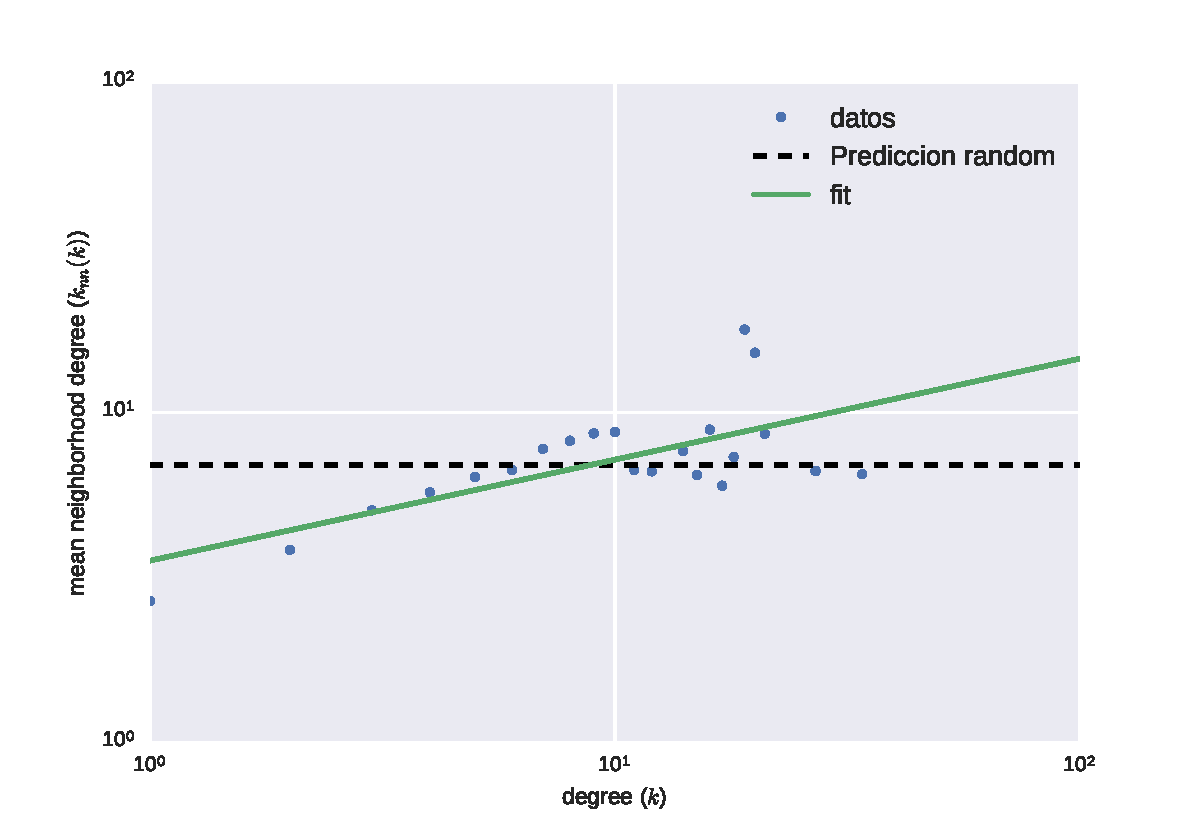
\includegraphics[width=\textwidth]{./schemes/assort_netscience-gml_loglog.pdf}
        \caption{\label{fig4:NETSCIENCE}NETSCIENCE}
    \end{subfigure}
    \begin{subfigure}[b]{0.45\columnwidth}
        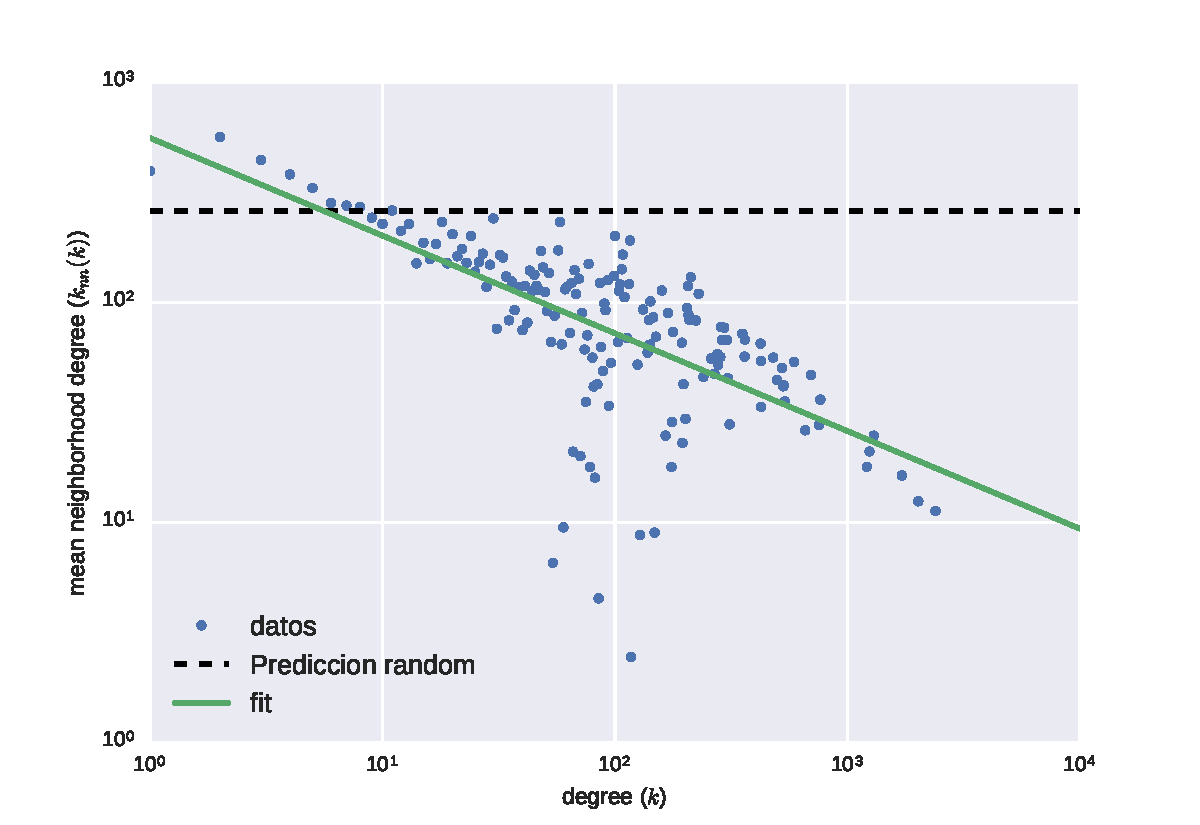
\includegraphics[width=\textwidth]{./schemes/assort_as-22july06-gml_loglog.pdf}
        \caption{\label{fig4:INTERNET}INTERNET}
    \end{subfigure}
    \\
    \begin{subfigure}[b]{0.45\columnwidth}
        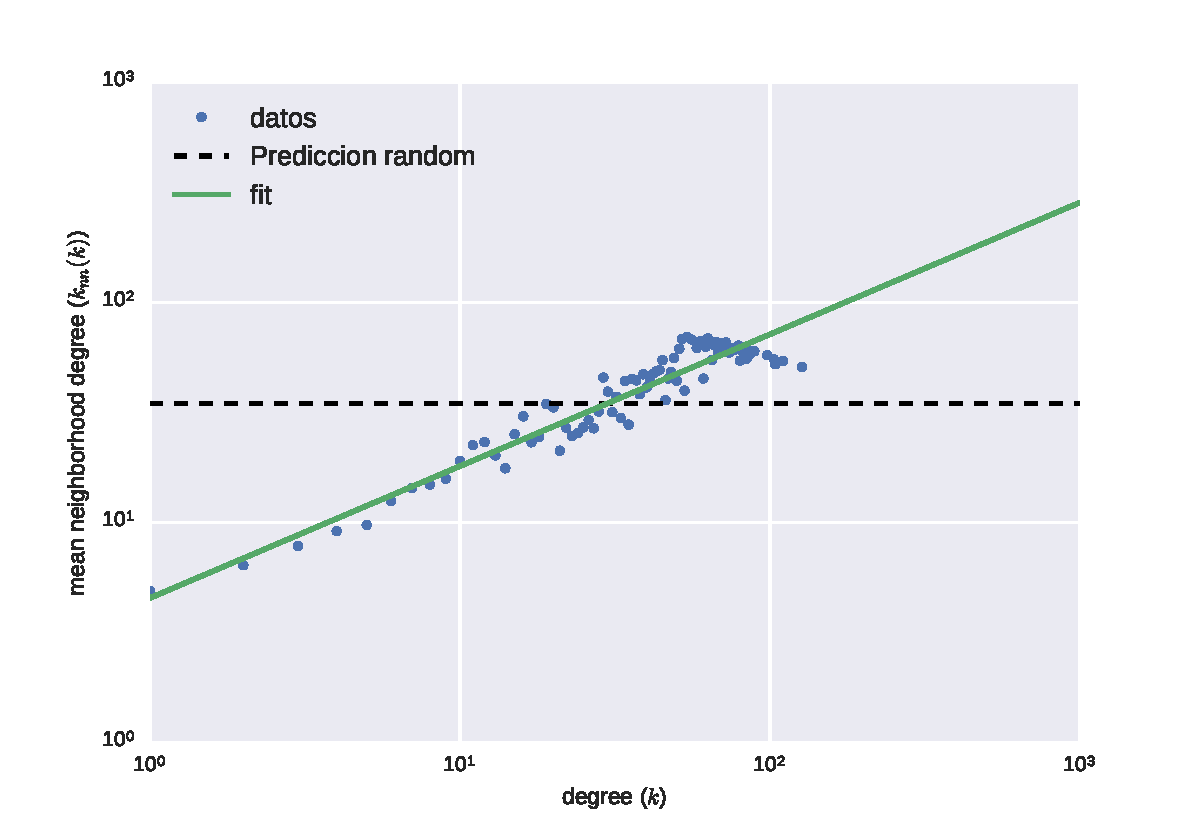
\includegraphics[width=\textwidth]{./schemes/assort_yeast_AP-MS-txt_loglog.pdf}
        \caption{\label{fig4:ap_ms} AP-MS}
    \end{subfigure}
    \begin{subfigure}[b]{0.45\columnwidth}
        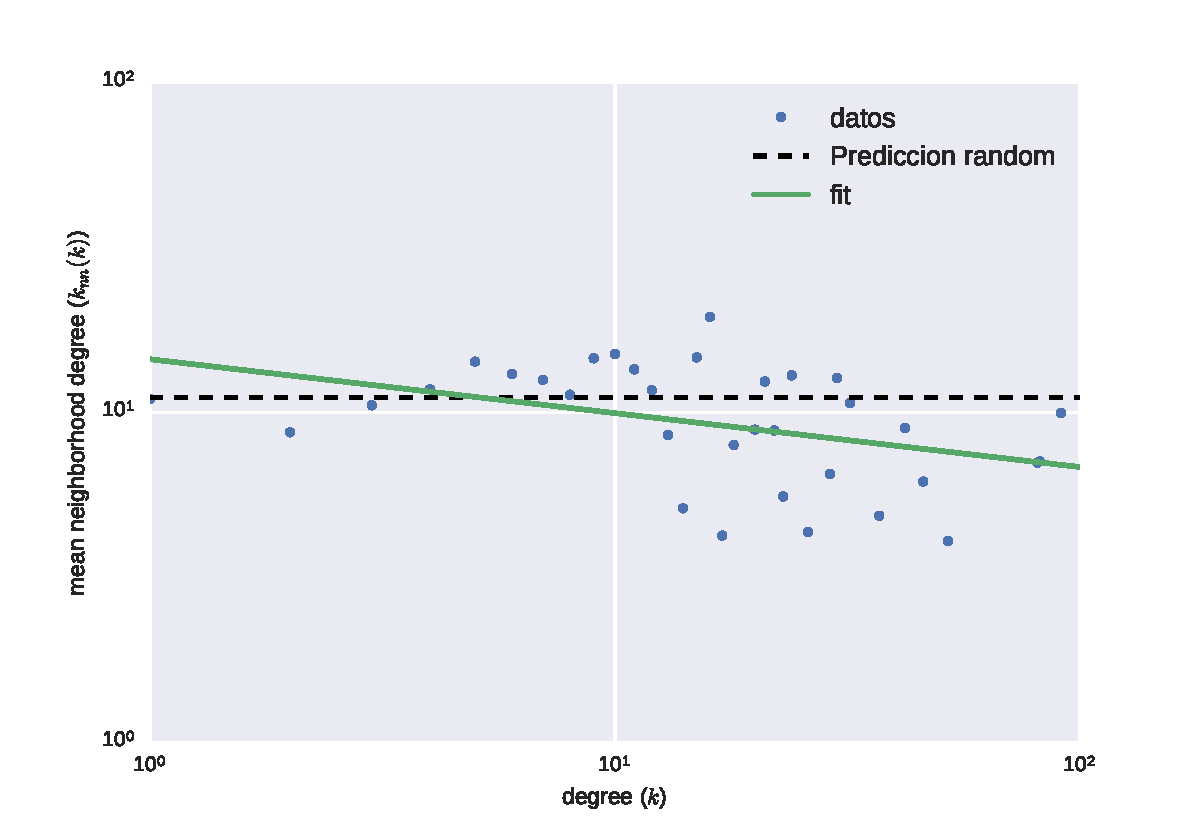
\includegraphics[width=\textwidth]{./schemes/assort_yeast_Y2H-txt_loglog.pdf}
        \caption{\label{fig4:y2h} Y2H}
    \end{subfigure}
    \caption{\label{fig4:mu} Grado medio del vecindario de $k$ para cada red en escala log-log. 
    Fiteo power law (Eq.~\ref{knn}) para cada caso: 
    (a) $\mu \approx 0.306 \pm 0.071$,
    (b) $\mu \approx -0.444 \pm 0.040$,
    (c) $\mu \approx 0.599 \pm 0.019$,
    (d) $\mu \approx -0.163 \pm 0.064$\\
    (script \texttt{assortivity\_powerlaw.py~<archivo>\quad-f <fmt>\quad-l}).}
\end{figure}



\subsection{Coeficiente de Correlaci\'on de Grado}
Por otro lado \citet{newman,newman2003} propuso un coeficiente de correlaci\'on de caracteristica $x$ (tambien llamado 
\textit{coeficiente de asortividad} ) dado por
\begin{align}
    r = \frac{\sum_{ij} \left( A_{ij} - k_i k_j/2m\right) x_i x_j}{\sum_{ij}k_i \delta_{ij} - k_i k_j/2m)x_i x_j}
    \label{r_general}
\end{align}
donde $x$ es la caracteristica una caracter\'istica del nodo, $A$ la matriz de adyacencia, $m$ el n\'umero total de links y $k_i$ el grado del nodo $i$. En el caso particular en que la caracteristica de interes es el grado del nodo, 
entonces la Ec. \ref{r_general} es

\begin{align}
    r = \frac{\sum_{ij} \left( A_{ij} - k_i k_j/2m\right) k_i k_j}{\sum_{ij}(k_i \delta_{ij} - k_i k_j/2m)k_i k_j}
    \label{r_k}
\end{align}

Cabe notar que en \citet{newman} se recomienda implementar de manera distinta para evitar exceso de computos n\'umericos. As\'i, 
tomando $  S_e = \sum_{ij} A_{ij} k_i k_j = 2\sum_{\text{links}(i,j)} k_i k_j $, 
$ S_1 = \sum_i k_i $, $ S_2 = \sum_i k_i^2 $ y $ S_3 = \sum_i k_i^3 $, y reemplazando en Ec.~\ref{r_k}

\begin{align}
    r &= \frac{S_1S_e - S_2^2}{S_1S_3 - S_2^2}
\end{align}

Una implementaci\'on del algoritmo descrito se puede encontrar en \texttt{assortative\_newman.py}. 

\subsection{Discusi\'on}

Para las redes estudiadas, la Tabla \ref{tab:assort} resume los resultados obtenidos 

\begin{table}[!ht]
    \centering
    \caption{\label{tab:assort} Tabla resumen de la asortatividad de las cuatro redes estudiadas.}
    {\scriptsize
    \begin{tabularx}{1\columnwidth}{XlX|XcXcXcX}
        \hline\hline
        & \multirow{2}{*}{Red}  &&& Tipo de     && \multirow{2}{*}{$\mu$}   && \multirow{2}{*}{$r$} &\\ 
        &                       &&& Asortividad &&                          &&                      &\\ 
        \hline
        & NETSCIENCE           &&& Asortativa   &&   0.306                  &&  0.461                &\\
        & INTERNET             &&& Disortativa  &&  -0.444                  && -0.198                &\\
        & AP-MS                &&& Asortativa   &&   0.599                  &&  0.461                &\\
        & Y2H                  &&& Disortativa  &&  -0.163                  && -0.041                &\\
        \hline\hline
    \end{tabularx}
    }
\end{table}

\citet{newman2003} reporta las asortatividad de 27 redes y obtiene que ciertos rangos de asortividad son caracteristicos del 
tipo de red en cuesti\'on, por ejemplo, por un lado redes biol\'ogicas suelen ser disortativas y por otro las redes sociales
tienen un comportamiento asortativo. En particular, en internet los  servidores (\textit{hubs}) no suelen conectarse 
entre ellos si no que m\'as bien reciben un gigantesco n\'umero de usuarios (nodos) y servidores peque\~nos, lo que explica
el comportamiento disortativo. Por otro lado, la red AP-MS est\'a construida a partir de medici\'on de afinidad, generando
grandes clusters altamente conectados entre ellos, est\'a manera de construir la red es probable que este asociada con la 
asortatividad reportada. Sin embargo, es necesario analizar rigurosamente tipo de asortatividad/disotatividad de estas redes
(si son disortatividades estructurales o no). Los ultimos dos casos (NETSCIENCE y Y2H) responden a los comportamientos
usuales para sus categor\'ias (redes sociales y biol\'ogicas respectivamente).

